\documentclass[tikz,border=5pt]{standalone}
\usepackage{amssymb,amsmath}
\newcommand{\C}{\mathbb{C}}
\newcommand{\CP}{\mathbb{CP}}
\newcommand{\Res}{\operatorname{Res}}
\begin{document}
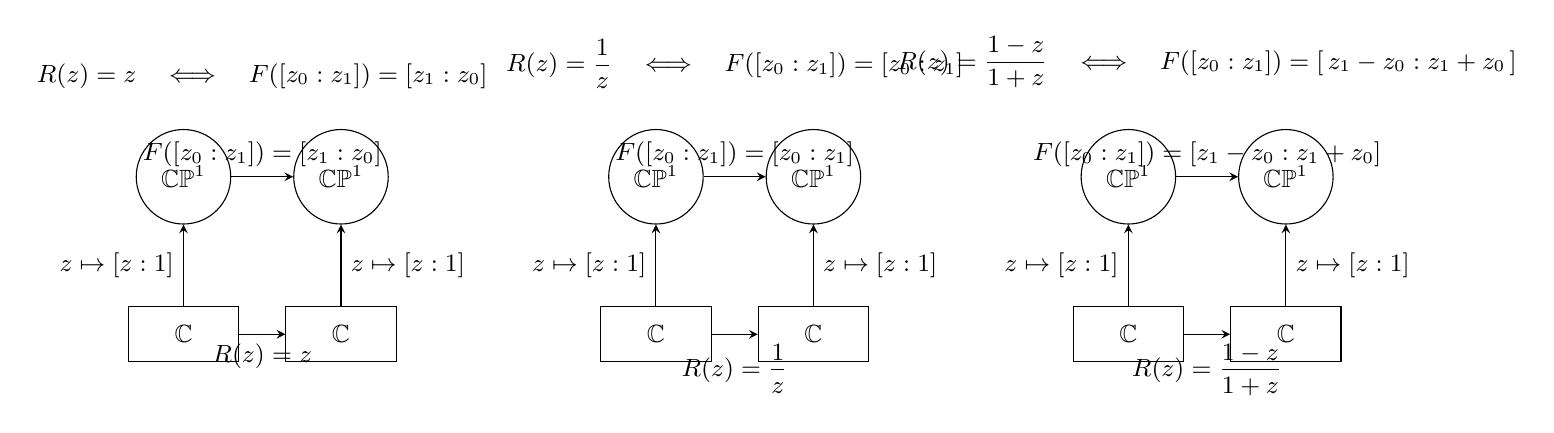
\begin{tikzpicture}[font=\small,>=stealth]
	
	% Style for CP^1 and C nodes
	\tikzset{
		cp1/.style={circle,draw,minimum width=1.2cm},
		cplane/.style={rectangle,draw,minimum width=1.4cm,minimum height=0.7cm}
	}
	
	%========================================
	% Diagram 1: R(z) = z  <->  F([z0:z1]) = [z1:z0]
	% (as written by the user)
	%========================================
	\begin{scope}[shift={(-6,0)}]
		
		% Title
		\node[above] at (0,2.0) {$R(z) = z \quad\Longleftrightarrow\quad
			F([z_0:z_1]) = [z_1:z_0]$};
		
		% Top: CP^1 -> CP^1
		\node[cp1] (CP1L1) at (-1,1) {$\CP^1$};
		\node[cp1] (CP1R1) at ( 1,1) {$\CP^1$};
		\draw[->] (CP1L1) -- (CP1R1)
		node[midway,above] {$F([z_0:z_1])=[z_1:z_0]$};
		
		% Bottom: C -> C
		\node[cplane] (CL1) at (-1,-1) {$\C$};
		\node[cplane] (CR1) at ( 1,-1) {$\C$};
		\draw[->] (CL1) -- (CR1)
		node[midway,below] {$R(z)=z$};
		
		% Vertical arrows: affine chart z = z0/z1
		\draw[->] (CL1) -- (CP1L1)
		node[midway,left] {\(\displaystyle z\mapsto[z:1]\)};
		\draw[->] (CR1) -- (CP1R1)
		node[midway,right] {\(\displaystyle z\mapsto[z:1]\)};
		
	\end{scope}
	
	%========================================
	% Diagram 2: R(z) = 1/z  <->  F([z0:z1]) = [z0:z1]
	% (as written by the user)
	%========================================
	\begin{scope}[shift={(0,0)}]
		
		% Title
		\node[above] at (0,2.0) {$R(z) = \dfrac{1}{z} \quad\Longleftrightarrow\quad
			F([z_0:z_1]) = [z_0:z_1]$};
		
		% Top: CP^1 -> CP^1
		\node[cp1] (CP1L2) at (-1,1) {$\CP^1$};
		\node[cp1] (CP1R2) at ( 1,1) {$\CP^1$};
		\draw[->] (CP1L2) -- (CP1R2)
		node[midway,above] {$F([z_0:z_1])=[z_0:z_1]$};
		
		% Bottom: C -> C
		\node[cplane] (CL2) at (-1,-1) {$\C$};
		\node[cplane] (CR2) at ( 1,-1) {$\C$};
		\draw[->] (CL2) -- (CR2)
		node[midway,below] {$R(z)=\dfrac{1}{z}$};
		
		% Vertical arrows: affine chart z = z0/z1
		\draw[->] (CL2) -- (CP1L2)
		node[midway,left] {\(\displaystyle z\mapsto[z:1]\)};
		\draw[->] (CR2) -- (CP1R2)
		node[midway,right] {\(\displaystyle z\mapsto[z:1]\)};
		
	\end{scope}
	
	%========================================
	% Diagram 3: R(z) = (1-z)/(1+z)  <->  F([z0:z1]) = [z1 - z0 : z1 + z0]
	%========================================
	\begin{scope}[shift={(6,0)}]
		
		% Title
		\node[above] at (0,2.0)
		{$R(z)=\dfrac{1-z}{1+z} \quad\Longleftrightarrow\quad
			F([z_0:z_1]) = [\,z_1 - z_0 : z_1 + z_0\,]$};
		
		% Top: CP^1 -> CP^1
		\node[cp1] (CP1L3) at (-1,1) {$\CP^1$};
		\node[cp1] (CP1R3) at ( 1,1) {$\CP^1$};
		\draw[->] (CP1L3) -- (CP1R3)
		node[midway,above]
		{$F([z_0:z_1]) = [z_1 - z_0 : z_1 + z_0]$};
		
		% Bottom: C -> C
		\node[cplane] (CL3) at (-1,-1) {$\C$};
		\node[cplane] (CR3) at ( 1,-1) {$\C$};
		\draw[->] (CL3) -- (CR3)
		node[midway,below] {$R(z)=\dfrac{1-z}{1+z}$};
		
		% Vertical arrows: affine chart z = z0/z1
		\draw[->] (CL3) -- (CP1L3)
		node[midway,left] {\(\displaystyle z\mapsto[z:1]\)};
		\draw[->] (CR3) -- (CP1R3)
		node[midway,right] {\(\displaystyle z\mapsto[z:1]\)};
		
	\end{scope}
	
\end{tikzpicture}
\end{document}
